\documentclass[11pt,a4paper]{article}
\usepackage{nabiadoc}
\usepackage{tikz}
\usetikzlibrary{positioning,arrows.meta,fit,calc}
\usepackage{caption}
\captionsetup[lstlisting]{justification=raggedright, singlelinecheck=false, font=small, labelfont=bf}
\usepackage{tabularx}

% Generated at build time by extract_snippets.py: excerpt locations, the MCP
% tool catalogue (tools.tex) and the AI configuration fields (config.tex).
\input{snippets.tex}
\newcommand{\snippetsource}[1]{\csname snippet@#1\endcsname}
\newcommand{\snippet}[3]{%
  \lstinputlisting[language=#2, caption={#3\\{\footnotesize\ttfamily\snippetsource{#1}}}]{#1.txt}}
% A prompt: plain text, wrapped.
\newcommand{\prompt}[2]{%
  \lstinputlisting[language={}, basicstyle=\ttfamily\scriptsize, keywordstyle={}, commentstyle={},
                   caption={#2\\{\footnotesize\ttfamily\snippetsource{#1}}}]{#1.txt}}
\lstset{basicstyle=\ttfamily\scriptsize, captionpos=t, numbers=none, aboveskip=8pt, belowskip=8pt,
        tabsize=4, keepspaces=true, breaklines=true, postbreak=\mbox{\textcolor{gray}{$\hookrightarrow$}\space}}
\renewcommand{\lstlistingname}{Code}
\newcommand{\sth}{\mathcal{S}}  % soft thresholding

% Pointers from a concept to its code.
\newcommand{\coderef}[1]{{\footnotesize\texttt{\snippetsource{#1}}}}
\newenvironment{codepointers}{%
  \par\smallskip\begingroup\footnotesize\noindent\textcolor{blue!50!black}{\textbf{Code}}\par\nopagebreak
  \begin{list}{}{\setlength{\leftmargin}{1.2em}\setlength{\itemsep}{0pt}\setlength{\parsep}{0pt}\setlength{\topsep}{1pt}}}%
  {\end{list}\endgroup\smallskip}
\newcommand{\codeitem}[2]{\item #2 --- \texttt{\snippetsource{#1}}}

% MCP tool catalogue entries (tools.tex).
\newcommand{\toolentry}[3]{\subsubsection*{\texttt{#1}}\vspace{-0.6em}
  \noindent{\footnotesize\textcolor{gray!30!black}{\emph{#2}\hfill\texttt{#3}}}\par\smallskip}
\newcommand{\modelentry}[2]{\subsubsection*{Input schema \texttt{#1}}\vspace{-0.6em}
  \noindent{\footnotesize\textcolor{gray!30!black}{\emph{pydantic model}\hfill\texttt{#2}}}\par\smallskip}
\newenvironment{toolparams}{\begin{description}\footnotesize\setlength{\itemsep}{0pt}\setlength{\parsep}{0pt}}{\end{description}}
% A reference to a section of another project's document.
\newcommand{\xref}[2]{\emph{#2} (#1 reference)}

\title{nabia Python: Package, Examples and Reference\\[0.3em]
\large Research on the nabia C++ library from Python}
\author{nabia documentation}
\date{October 2026}

\begin{document}
\maketitle

\begin{abstract}
This document is the reference for the Python project of nabia (\code{python/}): the
\code{nabia} package and the examples, built on the \code{nabia\_python\_bridge} wheel of the C++
project. It covers:
\begin{itemize}
  \item installing the wheel and using the whole C++ library from Python;
  \item portfolio backtests on pandas data (\code{nabia.backtest}, \code{nabia.latest\_weights});
  \item the analytics computed on price frames (\code{nabia.analytics}): correlations,
        volatilities, trend signals, drawdowns and the market regime;
  \item the market data pipeline (\code{nabia.marketdata});
  \item six worked examples on market data, which together use every function of the bridge.
\end{itemize}
The methods themselves are derived in the C++ reference (\code{cpp/doc}); the agents and the web
application that use this package are in the web UI reference (\code{webui/doc}). Excerpts and
code locations are extracted from the source when the document is built.
\end{abstract}

\tableofcontents
\clearpage
%==============================================================================
\part{Overview}

\section{Purpose and layout}\label{sec:architecture}
The Python project is where nabia is used for research: it loads market data, runs the C++
engines on pandas objects and plots the results. It contains no C++: the library comes from
the \code{nabia\_python\_bridge} wheel, built by the C++ project into \code{dist/}.
\begin{figure}[ht]
\centering
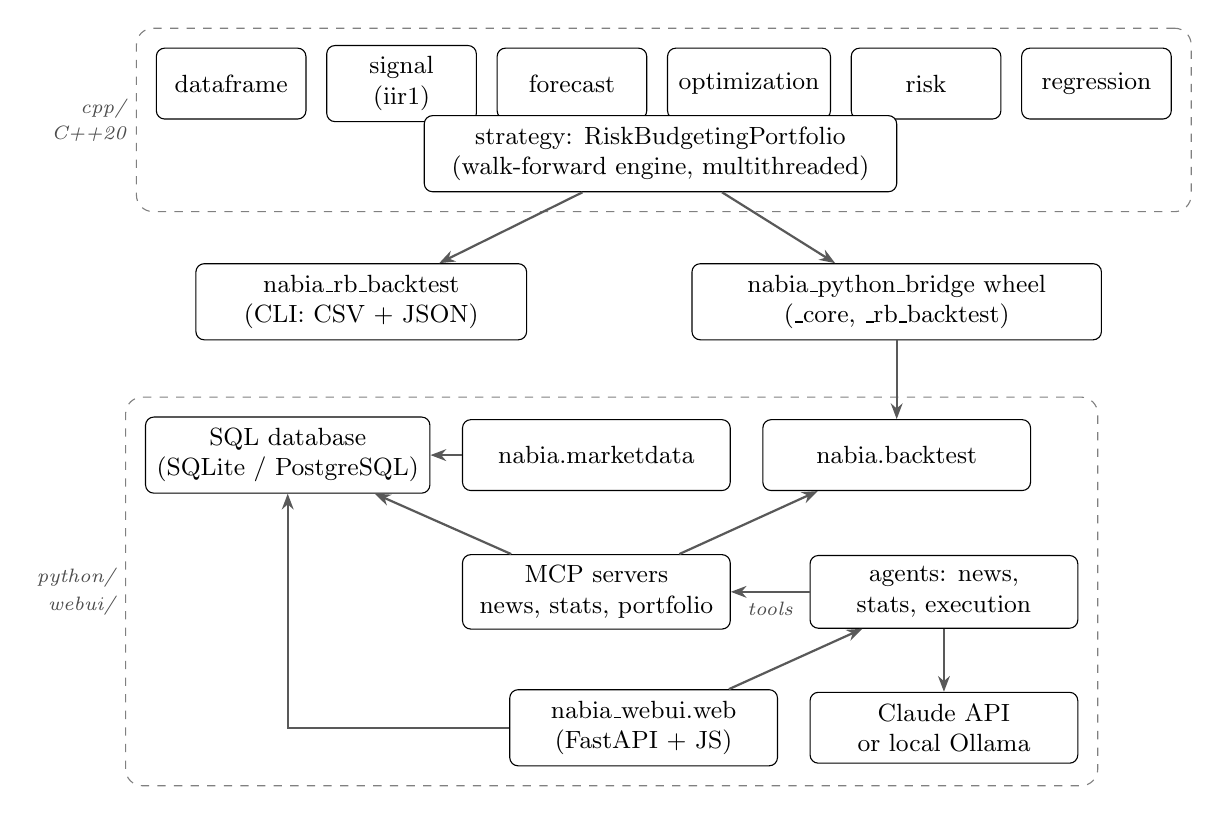
\begin{tikzpicture}[
  box/.style={draw, rounded corners=3pt, align=center, minimum height=9mm, font=\small, fill=white, inner sep=4pt},
  layer/.style={draw, dashed, rounded corners=6pt, inner sep=7pt, gray},
  arrow/.style={-{Stealth[length=2mm]}, thick, gray!70!black},
  lbl/.style={font=\scriptsize\itshape, gray!60!black}]
  \node[box, minimum width=19mm] (df) {dataframe};
  \node[box, right=2.5mm of df, minimum width=19mm] (sig) {signal\\(iir1)};
  \node[box, right=2.5mm of sig, minimum width=19mm] (fc) {forecast};
  \node[box, right=2.5mm of fc, minimum width=19mm] (opt) {optimization};
  \node[box, right=2.5mm of opt, minimum width=19mm] (risk) {risk};
  \node[box, right=2.5mm of risk, minimum width=19mm] (reg) {regression};
  \node[box, below=4mm of $(fc)!0.5!(opt)$, minimum width=60mm] (strat) {strategy: RiskBudgetingPortfolio\\(walk-forward engine, multithreaded)};
  \node[layer, fit=(df)(reg)(strat), label={[lbl]left:\shortstack[r]{cpp/\\C++20}}] (core) {};
  \node[box, below=9mm of strat, xshift=-38mm, minimum width=42mm] (cli) {nabia\_rb\_backtest\\(CLI: CSV + JSON)};
  \node[box, below=9mm of strat, xshift=30mm, minimum width=52mm] (bind) {nabia\_python\_bridge wheel\\(\_core, \_rb\_backtest)};
  \node[box, below=10mm of bind, minimum width=34mm] (pf) {nabia.backtest};
  \node[box, left=4mm of pf, minimum width=34mm] (md) {nabia.marketdata};
  \node[box, left=4mm of md, minimum width=30mm] (db) {SQL database\\(SQLite / PostgreSQL)};
  \node[box, below=8mm of md, minimum width=34mm] (mcp) {MCP servers\\news, stats, portfolio};
  \node[box, right=10mm of mcp, minimum width=34mm] (agents) {agents: news,\\stats, execution};
  \node[box, below=8mm of agents, minimum width=34mm] (llm) {Claude API\\or local Ollama};
  \node[box, left=4mm of llm, minimum width=34mm] (web) {nabia\_webui.web\\(FastAPI + JS)};
  \node[layer, fit=(db)(pf)(mcp)(agents)(llm)(web), label={[lbl]left:\shortstack[r]{python/\\webui/}}] (py) {};
  \draw[arrow] (strat) -- (cli);
  \draw[arrow] (strat) -- (bind);
  \draw[arrow] (bind) -- (pf);
  \draw[arrow] (md) -- (db);
  \draw[arrow] (mcp) -- (db);
  \draw[arrow] (mcp) -- (pf);
  \draw[arrow] (agents) -- node[lbl, below]{tools} (mcp);
  \draw[arrow] (agents) -- (llm);
  \draw[arrow] (web) -- (agents);
  \draw[arrow] (web.west) -| (db.south);
\end{tikzpicture}
\caption{The whole system and its three projects. Arrows point from a component to what it uses.}
\label{fig:architecture}
\end{figure}
\subsection{Three projects}
The repository holds three independent projects. Each opens on its own in an IDE, and each
has its own documentation in a \code{doc} folder:
\begin{center}\small
\begin{tabularx}{\linewidth}{@{}l l X@{}}
\toprule
Folder & IDE & Contents \\
\midrule
\code{cpp/} & CLion (CMake) & the C++ library (\code{include}, \code{src}), its tests, the
  command-line application, and the pybind11 bindings that build the
  \code{nabia\_python\_bridge} wheel into \code{dist/} \\
\code{python/} & PyCharm & the \code{nabia} package (backtests, analytics, market data) on top of
  the wheel, the examples, and the Python tests including the bridge tests \\
\code{webui/} & PyCharm & \code{nabia\_webui}: the agents, their MCP servers and the web app, on
  top of the \code{nabia} package \\
\bottomrule
\end{tabularx}
\end{center}
The projects depend on each other only through installed packages: \code{cpp} builds the wheel,
\code{python} installs it (\code{python/scripts/setup\_env.sh}), and \code{webui} installs both the
wheel and \code{python} in editable mode (\code{webui/scripts/setup\_env.sh}). Shared data, the market
database \code{data/market.db}, is at the repository root.

\subsection{Directory map}
\begin{center}\small
\begin{tabular}{@{}l>{\raggedright\arraybackslash}p{10cm}@{}}
\toprule
Path (in \code{python/}) & Contents \\
\midrule
\code{nabia/portfolio.py} & \code{backtest}, \code{latest\_weights} on pandas prices (\S\ref{sec:bindings}) \\
\code{nabia/analytics.py} & statistics on price frames (\S\ref{sec:stats}) \\
\code{nabia/marketdata} & universe, sources, SQL store, incremental download (\S\ref{sec:marketdata}) \\
\code{examples} & the worked examples and their data and plotting helpers (\S\ref{sec:examples}) \\
\code{tests} & pytest suites; \code{tests/bridge} tests the wheel itself \\
\code{scripts/setup\_env.sh} & creates \code{.venv} with the wheel and this package \\
\code{doc} & this reference (LaTeX source, PDF, \code{build.sh}) \\
\bottomrule
\end{tabular}
\end{center}

\subsection{Environment}
\begin{lstlisting}[language=bash]
cpp/scripts/build_wheels.sh 3.14          # in the C++ project: the wheel, into dist/
python/scripts/setup_env.sh               # python/.venv: the wheel + nabia (editable) + extras
cd python && .venv/bin/python -m pytest   # 49 tests, 2 opt-in network tests skipped
\end{lstlisting}
In PyCharm, open \code{python/} and select \code{python/.venv} as the interpreter. After the
wheel is rebuilt, run \code{setup\_env.sh} again: it reinstalls the wheel every time. To debug
the C++ code under a Python script, build the wheel with
\code{NABIA\_WHEEL\_BUILD\_TYPE=RelWithDebInfo} and attach CLion's debugger to the Python process.

%==============================================================================
\part{The C++ library in Python}

\section{\texorpdfstring{\code{nabia\_python\_bridge}}{nabia\_python\_bridge}}\label{sec:bridge}
The wheel exposes every public class and function of the C++ library. How it is built, and how
the bindings handle parameters, threads and errors, is in the C++ reference
(\xref{C++}{The full library in Python}).
\subsection{Modules}
\begin{center}\small
\begin{tabularx}{\linewidth}{@{}l X@{}}
\toprule
Module & Contents \\
\midrule
\code{stats} & \code{mean}, \code{variance}, \code{stddev}, \code{autocorrelation}; \code{normal\_pdf/cdf/quantile} (vectorized) \\
\code{signal} & \code{EWMA}, \code{ButterworthBandPass} (streaming \code{process}, batch \code{apply}), \code{moving\_average}, \code{exponential\_moving\_average}, \code{diff} \\
\code{forecast} & \code{KalmanFilter} (local level, local linear trend, custom), \code{GaussianProcess} with squared exponential, Mat\'ern 5/2, periodic, sum and product kernels (\code{k1 + k2}, \code{k1 * k2}), \code{SimpleExponentialSmoothing}, \code{Forecast} \\
\code{optimization} & \code{LBFGS}, \code{AugmentedLagrangian}, \code{SQP}, \code{NelderMead}, \code{DifferentialEvolution} with Python objectives; \code{BoxConstraints}, \code{LinearConstraint} \\
\code{risk} & \code{Volatility}, \code{ValueAtRisk}, \code{ExpectedShortfall}, \code{RiskBudgeting} \\
\code{strategy} & \code{RiskBudgetingPortfolio}, \code{compute\_performance}, \code{equity\_curve}, \code{drawdown\_series} \\
\code{regression} & \code{ElasticNet}, \code{elastic\_net\_path}, \code{lambda\_max}, \code{lambda\_grid}, \code{RegressionEngine} (\xref{C++}{Elastic net factor regression}) \\
\code{frames} & pandas interface: \code{backtest}, \code{regress}, \code{performance}, \code{metrics\_dict} \\
\bottomrule
\end{tabularx}
\end{center}
The \code{TimeSeries} and \code{DataFrame} containers are not bound, because pandas does
their job in Python. Where an engine takes indexed data, \code{frames} maps the pandas index
to row positions and back.

\paragraph{Conventions.}
\begin{itemize}
  \item Arrays are numpy \code{float64}: vectors are 1-d, and matrices have one row per observation.
  \item Parameter structs take their fields as keyword arguments, and unknown names raise
        \code{AttributeError}: \code{signal.EWMAParams(alpha=0.2)}. Models also accept the fields
        directly: \code{signal.EWMA(alpha=0.2)}. \code{lambda} is spelled \code{lambda\_}.
  \item Enums are Python enums (\code{regression.SubsetSearch.Forward}); in \code{frames}, a member
        name also works (\code{risk\_measure="ValueAtRisk"}).
  \item \code{std::invalid\_argument} becomes \code{ValueError}, ``not fitted'' becomes
        \code{RuntimeError}, and an exception raised in a Python objective propagates out of
        \code{optimize()}.
  \item Fits, backtests, regressions and optimizations release the GIL; Python objectives take it
        back for each call, so \code{DifferentialEvolution(num\_threads > 1)} is safe.
\end{itemize}
\begin{lstlisting}[language=Python]
import nabia_python_bridge as nb
from nabia_python_bridge import frames

rb = nb.risk.RiskBudgeting(nb.risk.RiskBudgetingParams(budgets=[0.5, 0.3, 0.2]), nb.risk.Volatility(cov))
weights = rb.optimize()
reg = frames.regress(fund_returns, factor_returns, min_factors=1, max_factors=3, train_fraction=0.7)
\end{lstlisting}

\section{Portfolio backtests: \texorpdfstring{\code{nabia.backtest}}{nabia.backtest}}\label{sec:bindings}
\code{nabia.portfolio} runs the C++ portfolio engine through \code{\_rb\_backtest}, a module of
the wheel's package \code{nabia\_python\_bridge}. The module reuses the command-line
application's JSON parser: Python and the command line accept the same parameters with the same
error messages (\xref{C++}{Backtest bindings for the Python package}). Data crosses the boundary
in simple forms: dates as \code{int64} days since 1970-01-01, prices as a \code{float64} matrix,
and parameters as JSON text.

Two functions are exposed:
\begin{itemize}
  \item \code{nabia.backtest(prices, params, budget\_schedule=None)} returns a result with
        pandas frames and metrics;
  \item \code{nabia.latest\_weights(prices, params)} solves only the last rebalance. The agents of
        the web UI use it to turn budgets into target weights.
\end{itemize}
\snippet{py_backtest_inputs}{Python}{pandas to C++}
\begin{codepointers}
  \codeitem{py_backtest}{Python \code{backtest}}
  \codeitem{py_latest_weights}{Python \code{latest\_weights}}
  \codeitem{py_to_days}{dates to day numbers}
\end{codepointers}

%==============================================================================
\part{Data and analytics}

\section{Market data}\label{sec:marketdata}

\subsection{Universe and sources}
The default download universe has four asset classes:
\begin{itemize}
  \item equity indices: S\&P 500, Nasdaq 100, Russell 2000, Euro Stoxx 50, DAX, FTSE 100,
        Nikkei 225, Hang Seng;
  \item US Treasury futures: 2Y, 5Y, 10Y, Bond, Ultra Bond;
  \item commodity futures: WTI, Brent, natural gas, gold, silver, copper, corn, wheat,
        soybeans;
  \item crypto against USD: BTC, ETH, SOL, XRP, ADA, LTC.
\end{itemize}
The AI portfolio uses the nine assets of Table~\ref{tab:universe-default}.

\begin{table}[ht]\centering\small
\caption{Default AI portfolio universe.}\label{tab:universe-default}
\begin{tabular}{@{}lll@{}}
\toprule
Symbol & Asset & Class \\
\midrule
\code{\textasciicircum GSPC} & S\&P 500 & equity index \\
\code{\textasciicircum STOXX50E} & Euro Stoxx 50 & equity index \\
\code{\textasciicircum N225} & Nikkei 225 & equity index \\
\code{ZN=F} & US 10-Year T-Note future & bond future \\
\code{ZB=F} & US Treasury Bond future & bond future \\
\code{BZ=F} & Brent crude oil future & commodity \\
\code{GC=F} & Gold future & commodity \\
\code{HG=F} & Copper future & commodity \\
\code{BTC/USD} & Bitcoin & crypto \\
\bottomrule
\end{tabular}
\end{table}

\paragraph{Sources.}
\begin{itemize}
  \item \textbf{Yahoo Finance} (\code{yfinance}) provides indices and futures, in batches.
        Futures are front-month continuous series, which jump at contract rolls. WTI
        settled negative on 2020-04-20, where simple returns are undefined, so the
        portfolio uses Brent.
  \item \textbf{Crypto exchanges} (\code{ccxt}, Coinbase by default) provide daily
        candles from public data, with no key. History is paged in windows of 300 candles.
        Windows before a coin's listing date are empty and are stepped over. Paging stops
        if the exchange ignores the start date.
\end{itemize}
\snippet{crypto_fetch}{Python}{Crypto daily candles with pagination}

\subsection{Storage and incremental updates}
Prices are stored per (symbol, date): open, high, low, close, adjusted close and volume.
\begin{itemize}
  \item \textbf{Upserts.} Writes use \code{INSERT ... ON CONFLICT DO UPDATE}, in the SQLite
        or PostgreSQL dialect, so re-downloading is idempotent and picks up revisions.
  \item \textbf{Incremental updates.} A stored symbol is re-fetched from five days before
        its last date, which corrects recent revisions.
  \item \textbf{Batching.} Symbols are grouped by source and start date.
\end{itemize}
\snippet{upsert_rows}{Python}{Portable upsert}
\snippet{update_market_data}{Python}{Incremental download}
\begin{codepointers}
  \codeitem{universe}{universe}
  \codeitem{yahoo_fetch}{Yahoo source}
  \codeitem{load_prices}{loading a price matrix}
\end{codepointers}

\section{Analytics on price frames}\label{sec:stats}
\code{nabia.analytics} computes the statistics the agents of the web UI see, and works on any
pandas frame of prices (dates by assets).

All statistics use daily close prices up to \code{as\_of}, over
\code{stats\_history\_days} (400) calendar days. Volatilities are annualized with
$\sqrt{252}$, standard deviations are sample standard deviations, and returns are simple
returns.
\begin{description}
  \item[Aligned returns] keep the dates where all assets have a price, then take returns.
        They are used for correlations only. Single-asset statistics use each asset's own
        history.
  \item[Correlation] is the Pearson correlation matrix $\rho$ of the last $w$ aligned
        returns (60 by default, at least 3). The \emph{average correlation} is
        \[
          \bar\rho=\frac{1}{n(n-1)}\sum_{i\ne j}\rho_{ij}.
        \]
  \item[Rolling volatility] is
        $\sigma^{(w)}=\mathrm{sd}\big(r_{T-w+1..T}\big)\sqrt{252}$ for
        $w\in\{20,60,120\}$. The \emph{volatility percentile} is computed from the series
        $v_s$ of rolling 20-day standard deviations over the last 252 dates:
        \[
          \pi=\frac{1}{|v|}\sum_s\mathbf 1[v_s\le v_T].
        \]
        So $\pi=1$ means the highest of the year.
  \item[Past returns] $P_T/P_{T-n}-1$ for $n\in\{21,63,126,252\}$ observations
        (1, 3, 6 and 12 months).
  \item[Moving-average distance] $P_T/\overline P_n-1$, where $\overline P_n$ is the mean
        of the last $n\in\{50,200\}$ prices.
  \item[Volatility-scaled 12-1 momentum]
        \[
          m=\frac{P_{T-21}/P_{T-252}-1}{\mathrm{sd}(r_{T-251..T})\sqrt{252}} .
        \]
        It is the 11-month return ending one month ago, which skips the short-term
        reversal, measured in units of the asset's own annual volatility.
  \item[Drawdowns] over the last 253 prices: $D_t=1-P_t/\max_{s\le t}P_s$. The tools
        report the current value and the maximum.
  \item[Market regime] combines five numbers:
        \begin{itemize}
          \item $\bar\rho$ over 60 and over 252 aligned returns;
          \item the median volatility percentile;
          \item the share of assets above their 200-day average;
          \item the share of assets with a positive 12-month return.
        \end{itemize}
\end{description}
\snippet{trend_signals}{Python}{Trend signals}
\snippet{rolling_volatility}{Python}{Volatilities and their percentile}
\snippet{market_regime}{Python}{Market regime}
\begin{codepointers}
  \codeitem{correlation_matrix}{correlation matrix}
  \codeitem{average_correlation}{average correlation}
\end{codepointers}

\section{Worked examples on market data}\label{sec:examples}
\code{examples} has six numbered scripts on \code{nabia\_python\_bridge}. They run on daily
closes from Yahoo Finance, cached as CSV, with the shared market database
(\code{../data/market.db}) as an offline fallback. A seventh,
\code{risk\_budgeting\_from\_market\_data.py}, uses the \code{nabia} package end to end: download,
backtest and the weights to hold now. Run them from \code{python/} with \code{.venv/bin/python
examples/01\_factor\_replication.py}, or in PyCharm.
Together they use every name the bridge exports. Each script prints its results with
comments computed from the numbers, and saves its figures as PNG in
\code{examples/figures/}, opening them when the matplotlib backend is interactive.
\begin{center}\small
\begin{tabularx}{\linewidth}{@{}l X@{}}
\toprule
Script & Content and figures \\
\midrule
\code{01\_factor\_replication} & A fund built as $0.5$ Nasdaq 100 $+\,0.3$ gold $+\,0.2$ 10y notes, plus alpha and 2\% noise. The engine recovers $0.497/0.300/0.193$ out of 14 candidates, and the bootstrap flags a spurious fourth factor. Figures: lasso path, $R^2$ by subset size, validation curve, bootstrap intervals, replication out of sample, tracking error \\
\code{02\_risk\_parity\_and\_budgeting} & Equal weights against risk parity for volatility, VaR and ES, inverse volatility, and a 40/40/20 class budget. Figures: capital against risk shares, correlations, risk by measure \\
\code{03\_portfolio\_backtest} & Walk-forward risk parity variants against equal weights, and a budget tilt in 2022. Figures: equity and drawdowns, weights and risk shares through time, leverage under a volatility target \\
\code{04\_signals\_and\_stats} & Fat tails and volatility clustering, smoothers, the band-pass cycle, EWMA crossovers. Figures: density against the normal, tail ratios, autocorrelations, trend filters and rule equity \\
\code{05\_forecasting} & Kalman filters and SES on realized volatility, a local linear trend on gold, and Gaussian processes on natural gas, all scored on a holdout. Figures: forecasts with intervals, innovations, slope, kernels, Gram matrix \\
\code{06\_optimization} & Max-Sharpe with L-BFGS against the closed form, constrained mean-variance with AL and SQP, GARCH(1,1) with Nelder--Mead, and rule calibration with differential evolution. Figures: efficient frontier, GARCH volatility, objective surface with the DE optima \\
\bottomrule
\end{tabularx}
\end{center}
\snippet{examples_coverage}{Python}{Every exported name must appear in an example}
\begin{codepointers}
  \codeitem{examples_data}{data download, cache and fallback}
  \codeitem{examples_plots}{figure saving}
\end{codepointers}


%==============================================================================
\part{Verification and limitations}

\section{Verification}\label{sec:verification}
\begin{description}
  \item[Bridge] (\code{tests/bridge}, 34 tests): every module of \code{nabia\_python\_bridge}
        against closed forms and numpy, the binding semantics, and the check that the examples
        use the whole exported API. The C++ project's wheel scripts run them on every wheel.
  \item[Package] (\code{tests}, 15 tests): \code{nabia.backtest} against the command-line
        application on its own example (a copy in \code{tests/data}), schedules and errors; the
        market data store, sources and incremental download against fakes. Two opt-in tests
        (\code{NABIA\_NETWORK\_TESTS=1}) download live data.
  \item[This document] Its excerpts and code locations are extracted at build time.
\end{description}

\section{Limitations}\label{sec:limitations}
\begin{itemize}
  \item \textbf{Continuous futures} jump at rolls. Back-adjusted series would remove
        spurious returns.
  \item \textbf{Asynchronous closes} (Asia against US) bias same-day correlations downwards.
        Multi-day returns or synchronized prices would reduce the bias.
  \item \textbf{The wheel} must match the interpreter of \code{.venv}; build it for that Python
        version first.
\end{itemize}

\end{document}
